\documentclass[pdf,bluish,slideColor,colorBG]{prosper}
\hypersetup{pdfpagemode=FullScreen}
\usepackage{graphicx,color}
\def\baselinestretch{0.7}
\parindent 0.3in
\hyphenpenalty=10000
\tolerance=10000
\pagestyle{empty}

\title{Week 10: Quantitative Genetics}

\author{Joe Felsenstein}
\institution{Genome 562}

\definecolor{golden}{rgb}{1.0,0.8,0}

\begin{document}

\def\Prob{{\rm Prob\;}}
\def\prob{{\rm \;Prob\;}}

\maketitle

{\parindent=0in

%\begin{slide}[Replace]{John Burdon Sanderson Haldane (1892-1964) }
%
%\centerline{\includegraphics[width=1.5in]{Haldane2.ps}}
%\bigskip
%
%\centerline{Pictured in about 1940.}
%
% \end{slide}
% 
% \begin{slide}[Replace]{Motoo Kimura (1924-1994) }
% 
% \centerline{\includegraphics[width=2.0in]{kimura.ps}}
% \bigskip
% 
% \centerline{With his wife and son in the 1960s}
% 
% \end{slide}
% 
\begin{slide}[Replace]{The Biometricians}

\hspace*{0in} \hfill \includegraphics[width=1.5in]{galton.ps}
\hfill \includegraphics[width=1.5in]{pearson.ps} \hfill {~~}

\hspace*{0in} \hfill Francis Galton (1822-1911) \hfill Karl Pearson (1857-1936)
\hfill {~~}

\end{slide}

%\begin{slide}[Replace]{Francis Galton sees a law of heredity}
%
%\centerline{\includegraphics[width=2.0in]{galton-corr.ps}}
%\bigskip
%
%... or what he thinks is one.  These days we'd just say he saw a bivariate normal
%distribution.
%
%\end{slide}
%

\begin{slide}[Replace]{Ronald Aylmer Fisher (1890-1962) }
\bigskip


\begin{center}
\begin{tabular}{c c}
\includegraphics[height=1.8in]{Fisher.ps} &
\includegraphics[height=1.8in]{Fisher1952.ps}\\
about 1930 & in 1952 
\end{tabular}
\end{center}

\noindent
Fisher, R. A.  1918.  The correlation between relatives on the supposition of
mendelian inheritance.  {\it Philosophical
Transactions of the Royal Society of Edinburgh}, {\bf 52:} 399 -- 433.

\end{slide}

\begin{slide}[Replace]{A one-locus quantitative character}

\centerline{\includegraphics[width=1.4in]{fig9-1.ydraw}}

\end{slide}

\begin{slide}[Replace]{A two-locus quantitative character}

\centerline{\includegraphics[width=1.4in]{fig9-2.ydraw}}

\end{slide}

\begin{slide}[Replace]{Distributions with different numbers of loci}

\centerline{\includegraphics[width=2.4in]{fig9-7.ydraw}}
\bigskip

Each has a number of completely dominant loci (all of equal effect), with
size of effects scaled so that overall genetic variance is equal, and
with an environmental effect that contributes 20\% of the variation.

\end{slide}

\begin{slide}[Replace]{Regression of offspring on a parent}

\centerline{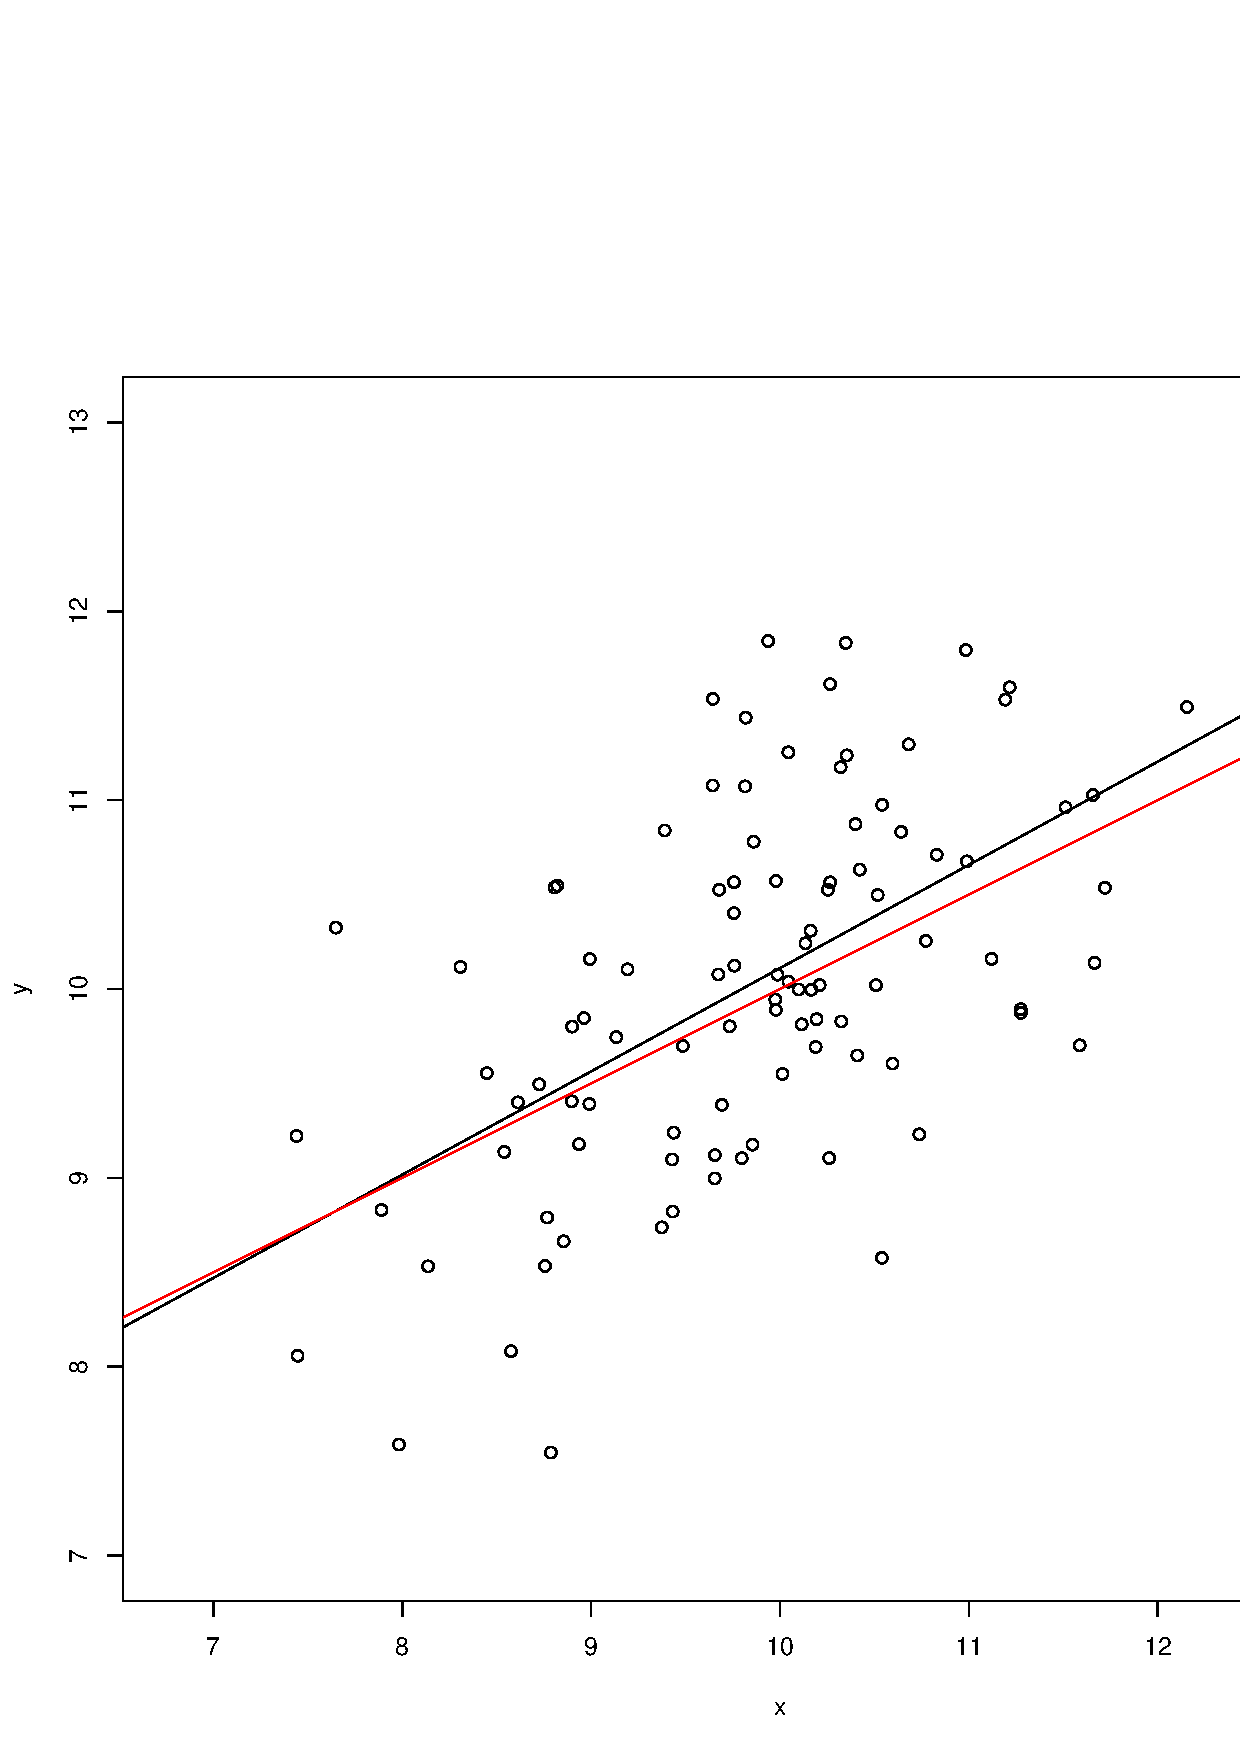
\includegraphics[width=2.8in]{fig9-5.idraw}}

\end{slide}

\begin{slide}[Replace]{Regression of offspring on a parent}

\centerline{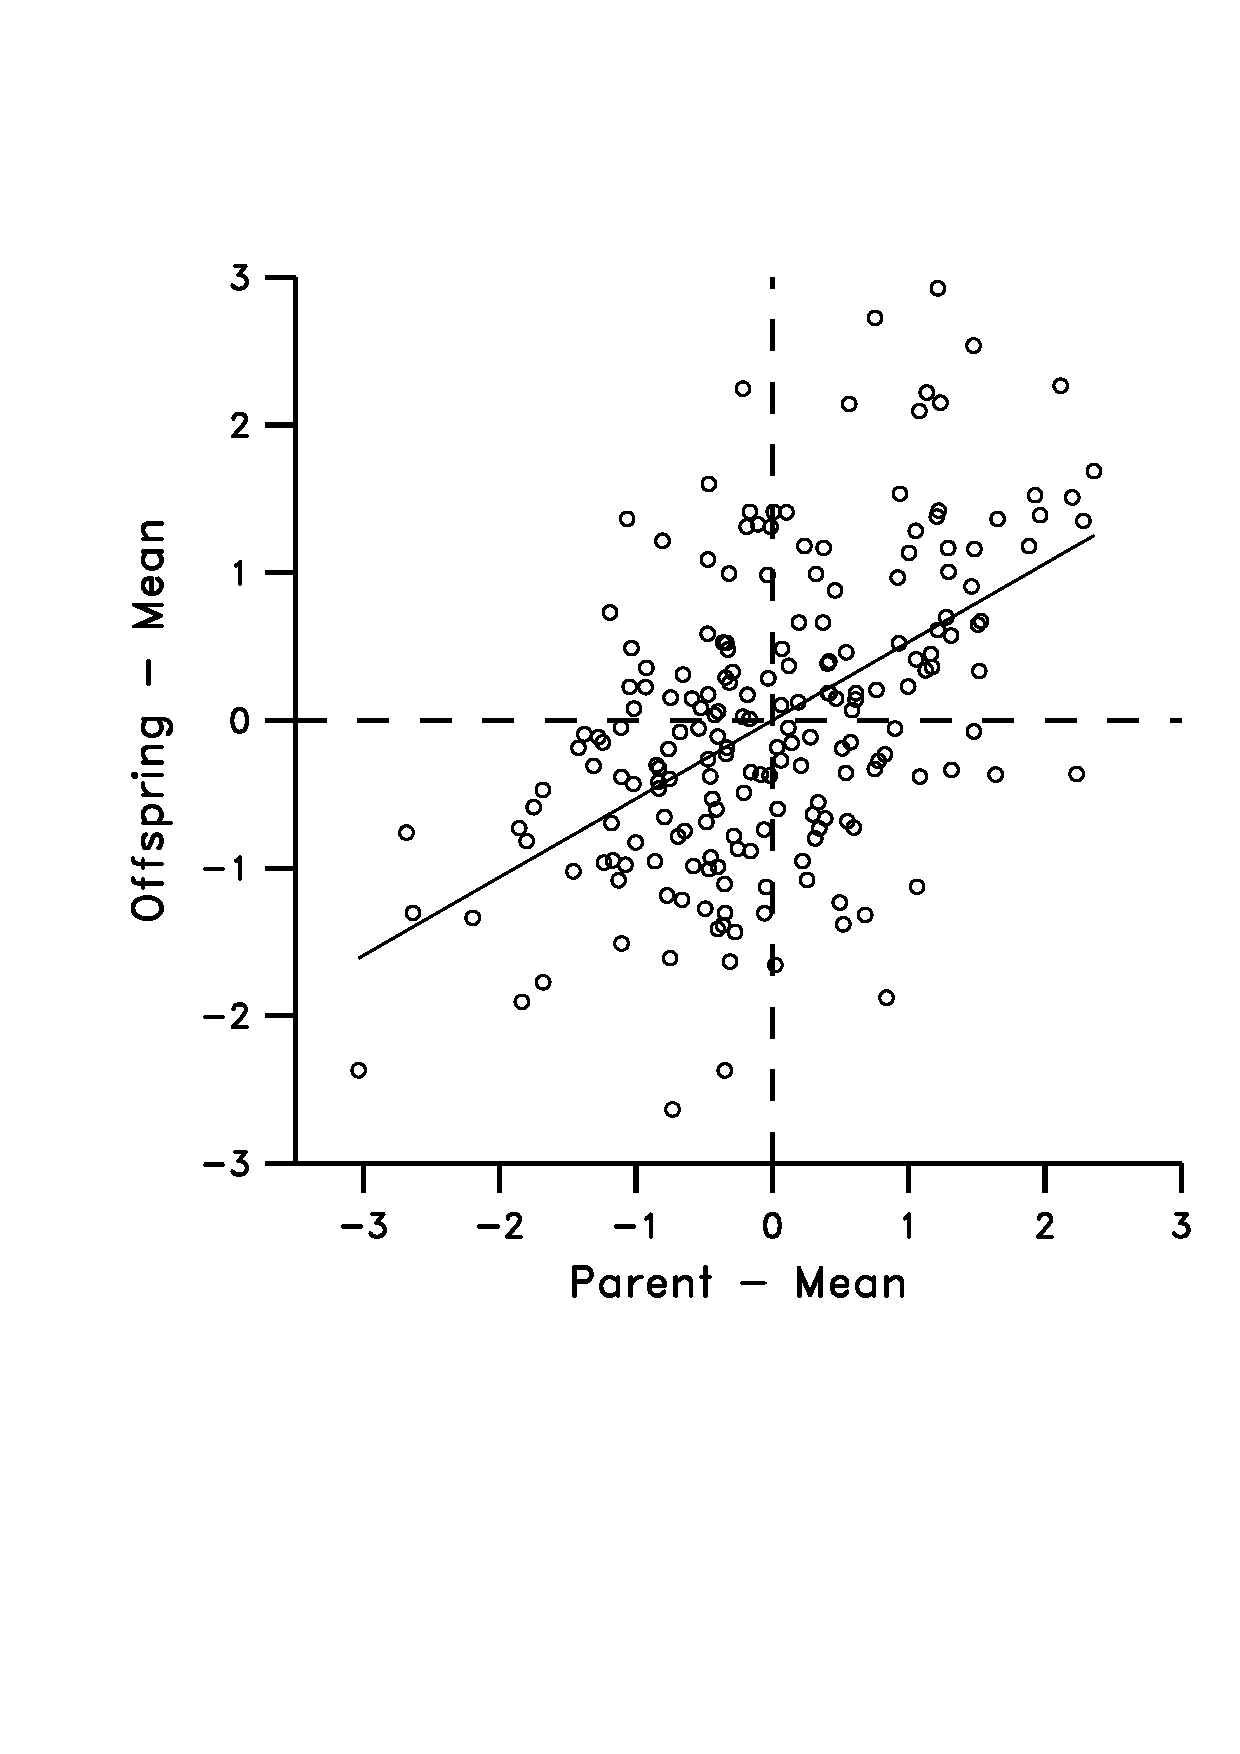
\includegraphics[width=2.8in]{fig9-6.idraw}}

\end{slide}

\begin{slide}[Replace]{Regression of effects at one locus on gene dose}

\centerline{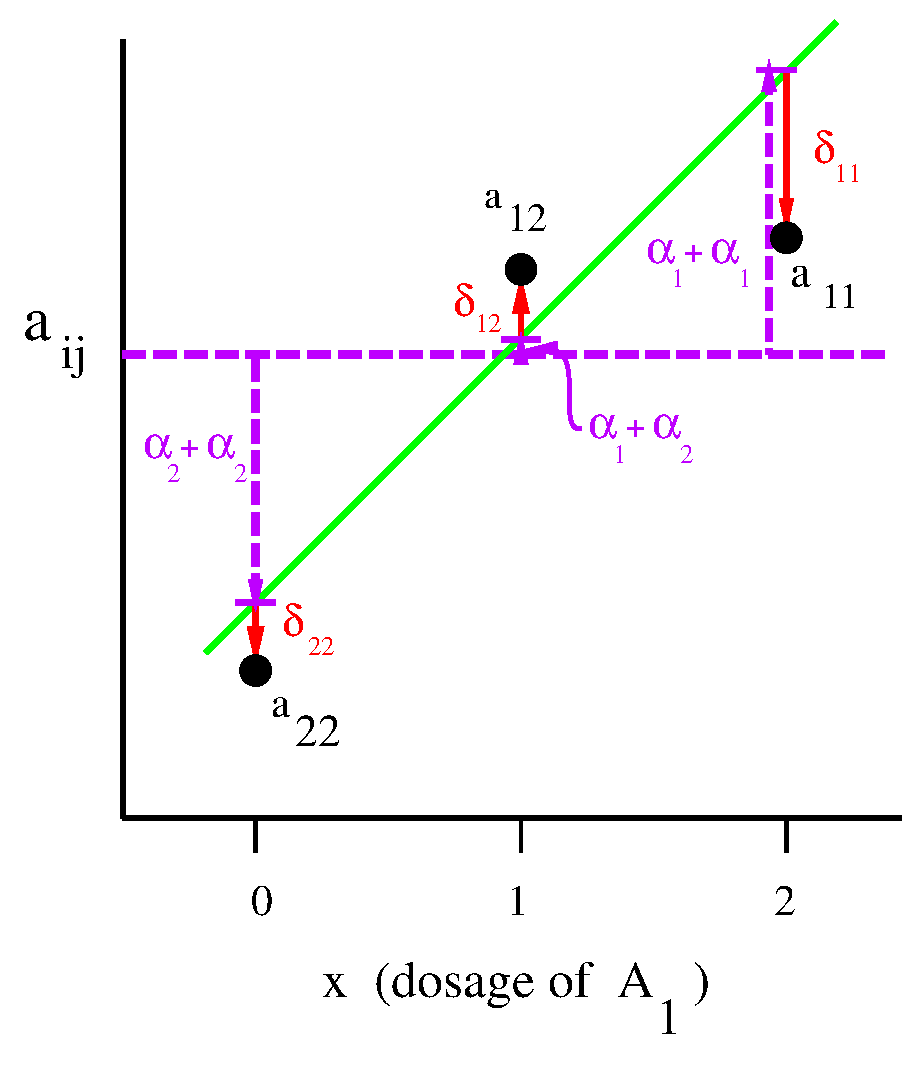
\includegraphics[width=2.8in]{fig9-3.ps}}

\end{slide}

%\begin{slide}[Replace]{Coefficients from parents and offspring}
%
%\centerline{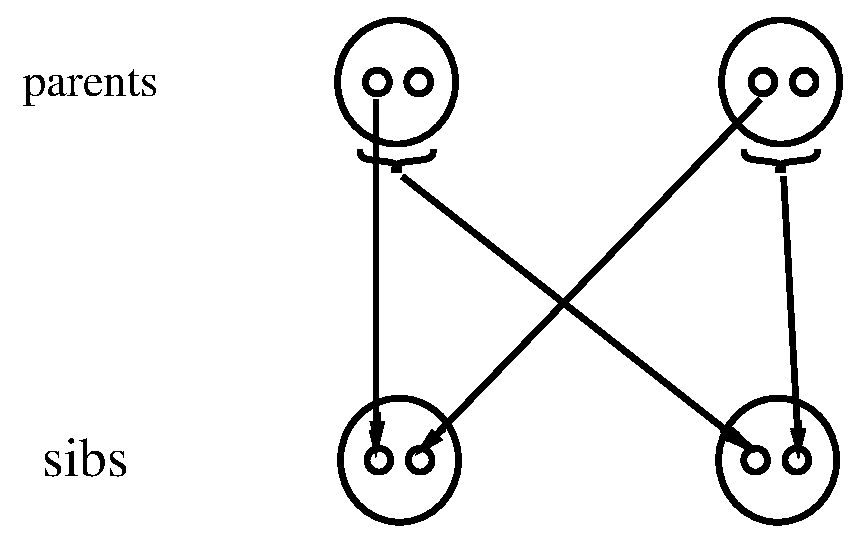
\includegraphics[width=3.3in]{fig9-4.ps}}
%
%\end{slide}
%
\begin{slide}[Replace]{Jay L. Lush (1896-1982) }
\bigskip

\begin{center}
\begin{tabular}{c c}
\includegraphics[height=1.5in]{Lush.ps} &
\includegraphics[height=1.5in]{Lush1945.ps}\\
about 1960 & {\it Animal Breeding Plans}
\end{tabular}
\end{center}

\bigskip


\end{slide}

}

\end{document}
